\documentclass[a4paper]{article}

\usepackage[pdftex]{graphicx}
\usepackage[margin=3cm]{geometry}
\usepackage{verbatim,moreverb,amssymb,amsmath,paralist,booktabs}
\usepackage[noend]{algorithmic}

\algsetup{indent=2em}
\renewcommand{\algorithmiccomment}[1]{\quad \{\emph{#1}\}}


\newcounter{question}
\newcommand{\question}[1]{\refstepcounter{question}\section*{Question~\thequestion~~~\small\emph{(#1)}}}
\renewcommand*\thequestion{\arabic{question}}


\begin{document}

\pagestyle{empty}
\thispagestyle{empty}



\noindent
\begin{minipage}{\columnwidth}
  \centering
  \Large
  DA4002 (HT13) Halmstad University\\
  Introduction to Algorithms, Data Structures, and Problem Solving\\[3\baselineskip]
  \Huge
  Written Exam\\
  \Large
  Saturday, January 11, 2014\\[2\baselineskip]
  Examiner: Roland Philippsen
\end{minipage}

\vfill

\noindent
\begin{center}
\fbox{
  \begin{minipage}{0.8\columnwidth}
    \textbf{Student Name:}\\[3\baselineskip]
  \end{minipage}
}
\end{center}

\vfill



\section*{Rules}

Aside from the obvious rules of conduct exams (e.g.\ no chatting):

\begin{itemize}
\item
  \textbf{No computing devices} (laptops, phones, calculators, \emph{etc}).
\item
  \textbf{No books or printouts} except for non-electronic dictionaries.
\item
  \textbf{Allowed hand-written notes}: two sheets of A4 paper (front and back).
\end{itemize}



\section*{General Guidelines}

\begin{itemize}
\item
  \textbf{Read carefully} and pace yourself.
  You can solve the problems in any order you want, but later problems may be easier to solve after you have answered the preceding questions.
\item
  \textbf{Write clearly} and draw clear diagrams.
  If you need to correct a mistake, then cleanly cross out the wrong answer and clearly indicate where the correction can be found.
\item
  \textbf{Indicate the question number} for each of your answers.
  If a question has sub-questions, indicate the sub-question number after the main question number, separated by a dot.
  For example, question 3 has 4 sub-questions, and their answers should be numbered 3.1, 3.2, 3.3, and 3.4.
\end{itemize}



\pagebreak
\pagestyle{plain}
\thispagestyle{plain}
\setcounter{page}{1}



\question{6 points}

A \textbf{queue} is a data structure where items can be appended and retrieved.
The oldest item that was appended to a queue is the next one to be retrieved.
A \textbf{stack} is a data structure where items can be pushed and popped.
The youngest item that was pushed is the next one to be popped.
A \textbf{priority queue} is a data structure which allows to insert and extract items based on a priority.
An extracted item always has the highest priority of all the items in the priority queue at that moment.

Each of the data structures can be implemented in various ways, for example using linked lists, vectors (dynamically sized arrays), heaps (array-backed balanced trees), or combinations such as arrays of lists.
Consider the following possibilities:

\begin{itemize}
\item
  Queue
  \begin{itemize}
  \item
    list-based ``append'' operation
  \item
    list-based ``retrieve'' operation
  \item
    vector-based ``append'' operation
  \item
    vector-based ``retrieve'' operation
  \end{itemize}
\item
  Stack
  \begin{itemize}
  \item
    list-based ``push'' operation
  \item
    list-based ``pop'' operation
  \item
    vector-based ``push'' operation
  \item
    vector-based ``pop'' operation
  \end{itemize}
\item
  Priority queue
  \begin{itemize}
  \item
    heap-based ``insert'' operation
  \item
    heap-based ``extract'' operation
  \item
    array-of-lists-based ``insert'' operation
  \item
    array-of-lists-based ``extract'' operation
  \end{itemize}
\end{itemize}

For each of the six functions given on the next page, write down which of the above 12 operations it implements.
You can write the function label (A, B, C, D, E, and F) beside the corresponding list items above.

\clearpage

\twocolumn
\small
\verbatiminput{shell.c}
\normalsize
\onecolumn



\clearpage
\question{6 points}

What is the runtime complexity for each of the following six programs?

\begin{center}
  \begin{tabular}{cccc}
    \toprule
    $T(N)$ & $T(N) / \log N$ & $T(N) / N$ & $T(N) / N^2$ \\
    \midrule
    \multicolumn{4}{l}{Program \textbf{A}} \\
    \quad
    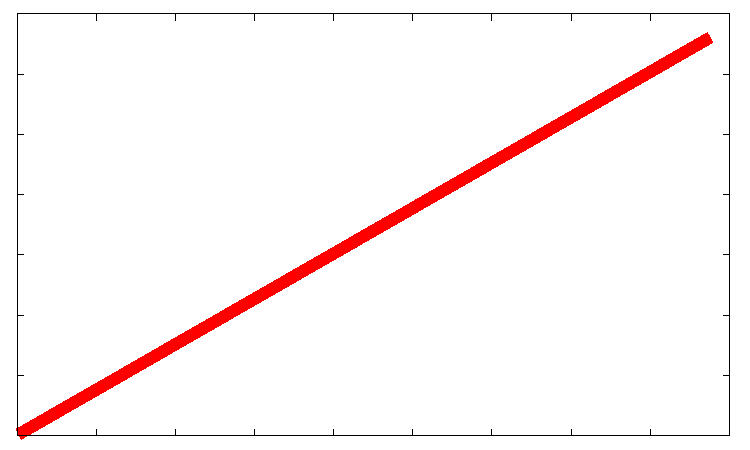
\includegraphics[width=0.23\columnwidth]{flin1.pdf} &
    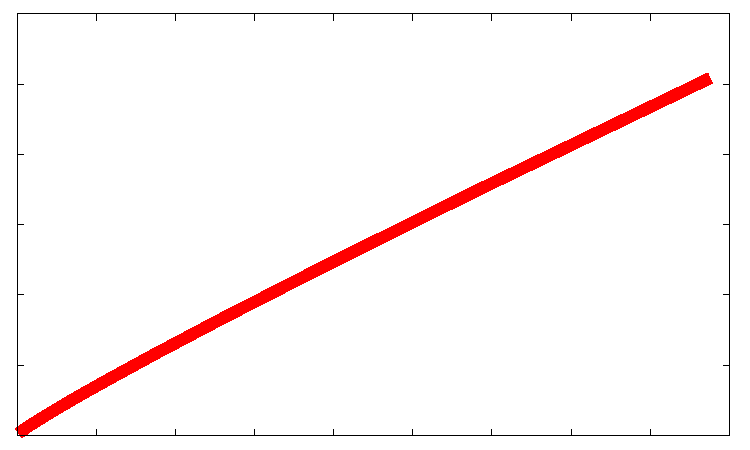
\includegraphics[width=0.23\columnwidth]{flin1-log.pdf} &
    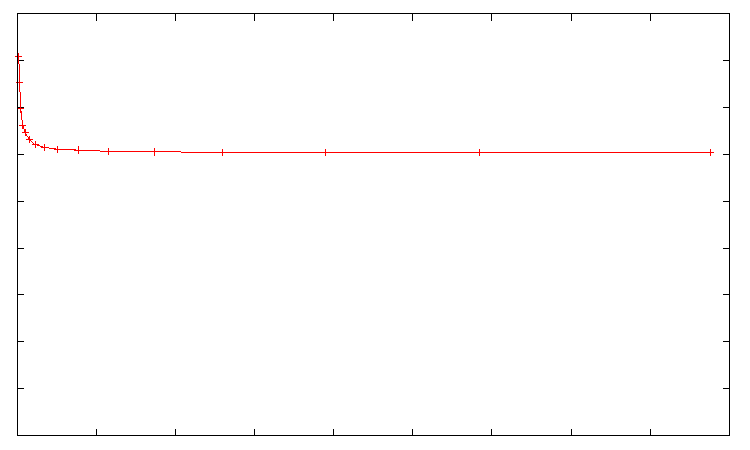
\includegraphics[width=0.23\columnwidth]{flin1-n.pdf} &
    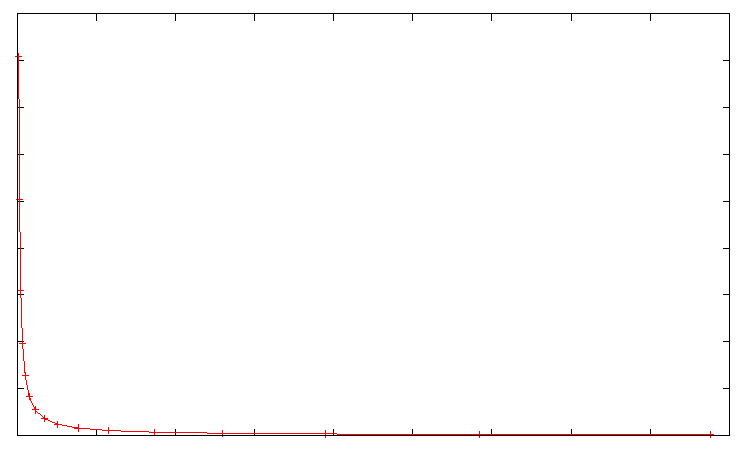
\includegraphics[width=0.23\columnwidth]{flin1-n2.pdf} \\
    \midrule
    \multicolumn{4}{l}{Program \textbf{B}} \\
    \quad
    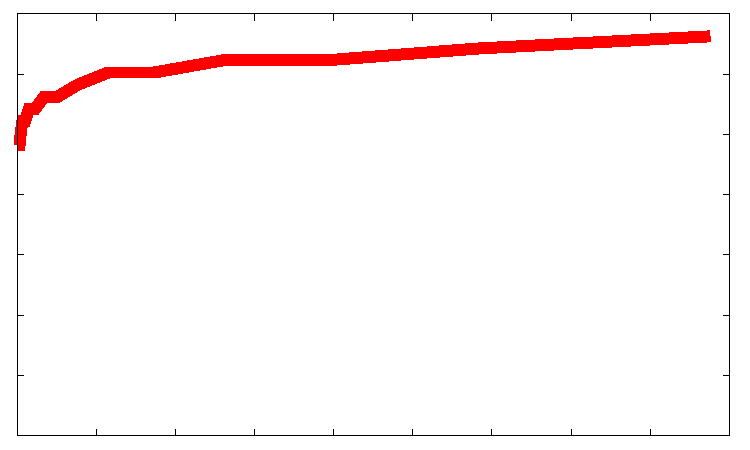
\includegraphics[width=0.23\columnwidth]{flog1.pdf} &
    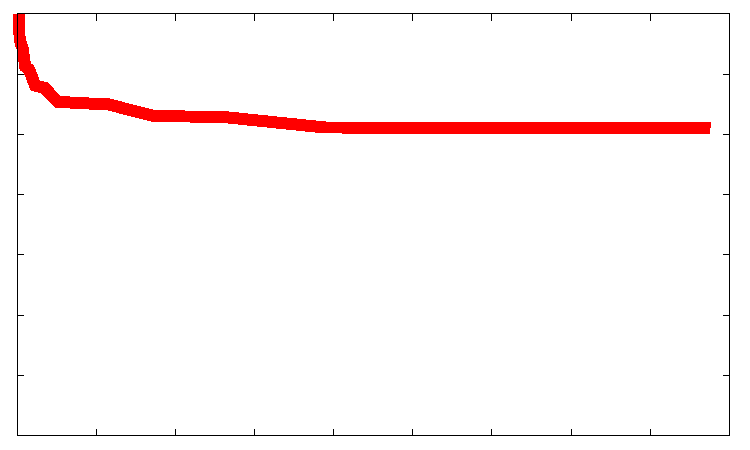
\includegraphics[width=0.23\columnwidth]{flog1-log.pdf} &
    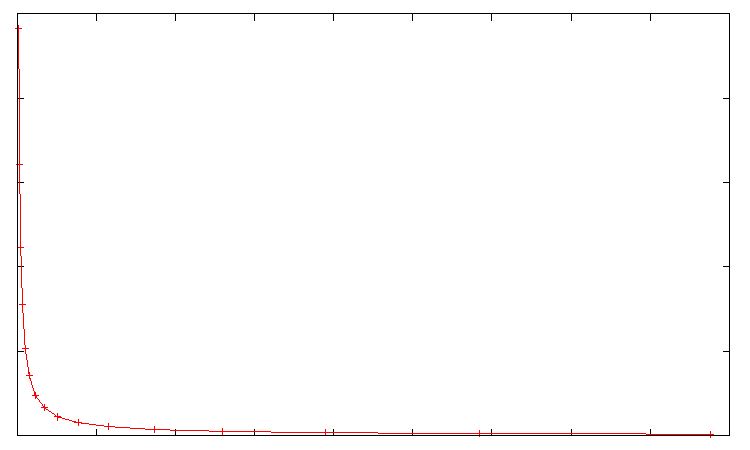
\includegraphics[width=0.23\columnwidth]{flog1-n.pdf} &
    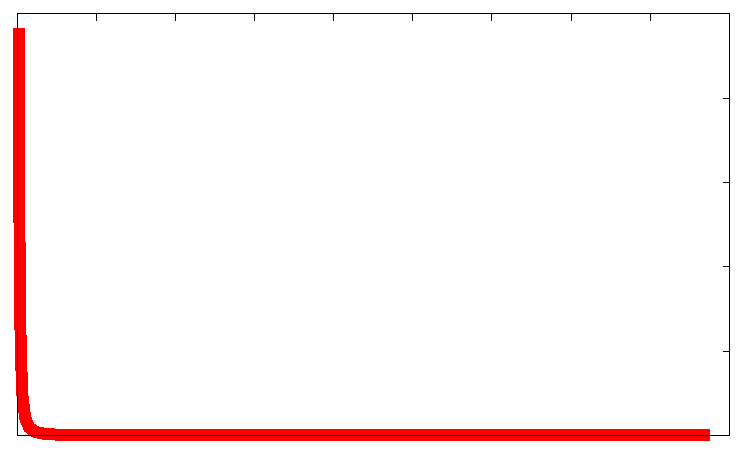
\includegraphics[width=0.23\columnwidth]{flog1-n2.pdf} \\
    \midrule
    \multicolumn{4}{l}{Program \textbf{C}} \\
    \quad
    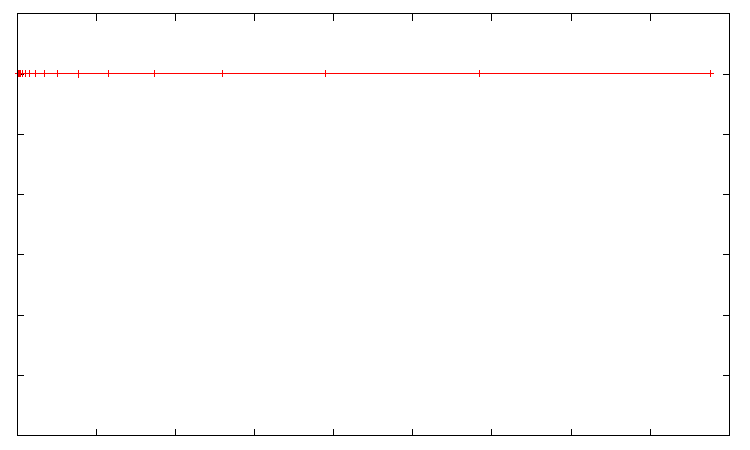
\includegraphics[width=0.23\columnwidth]{fconst.pdf} &
    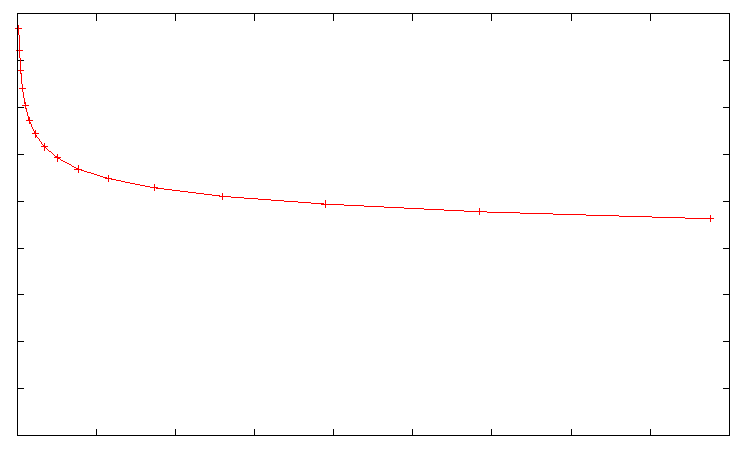
\includegraphics[width=0.23\columnwidth]{fconst-log.pdf} &
    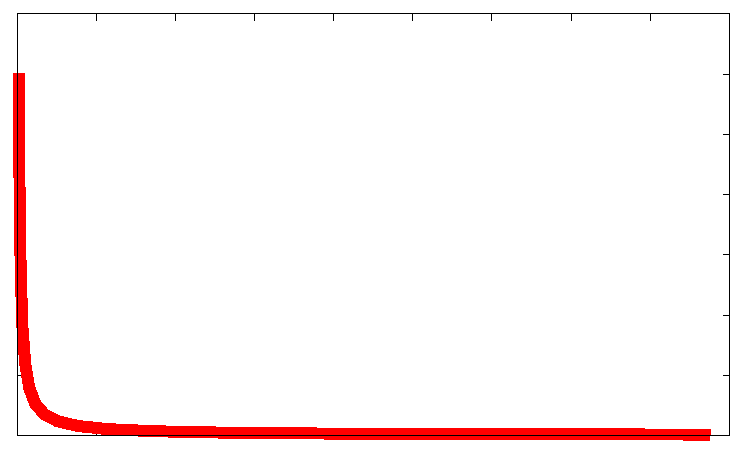
\includegraphics[width=0.23\columnwidth]{fconst-n.pdf} &
    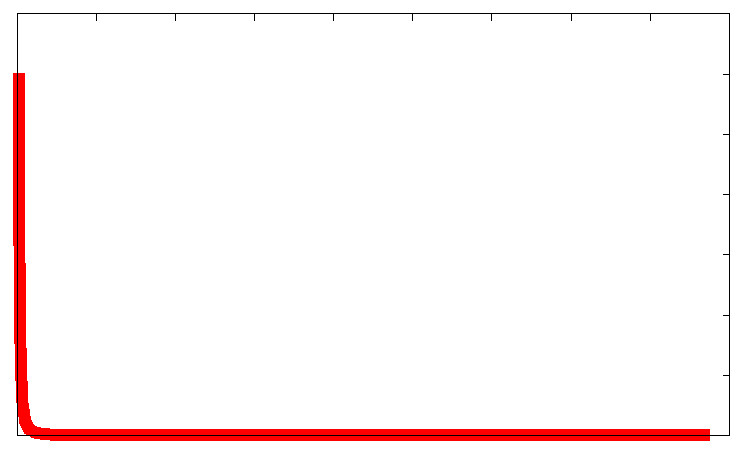
\includegraphics[width=0.23\columnwidth]{fconst-n2.pdf} \\
    \midrule
    \multicolumn{4}{l}{Program \textbf{D}} \\
    \quad
    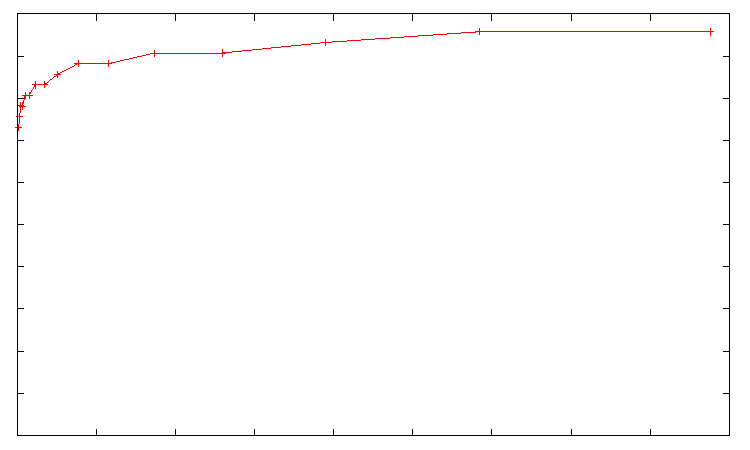
\includegraphics[width=0.23\columnwidth]{flog2.pdf} &
    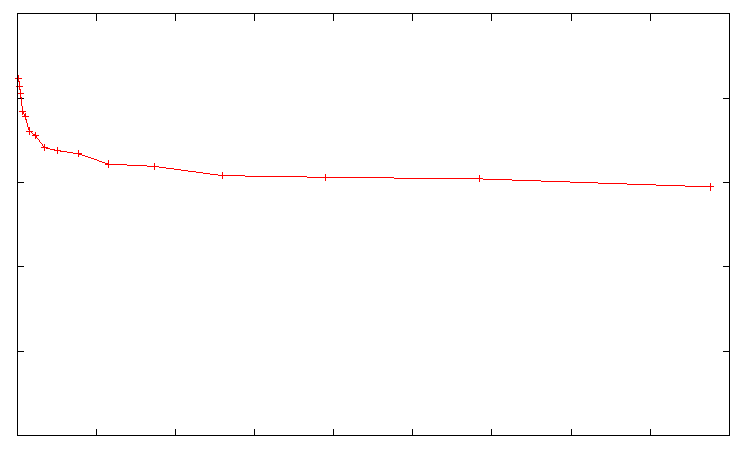
\includegraphics[width=0.23\columnwidth]{flog2-log.pdf} &
    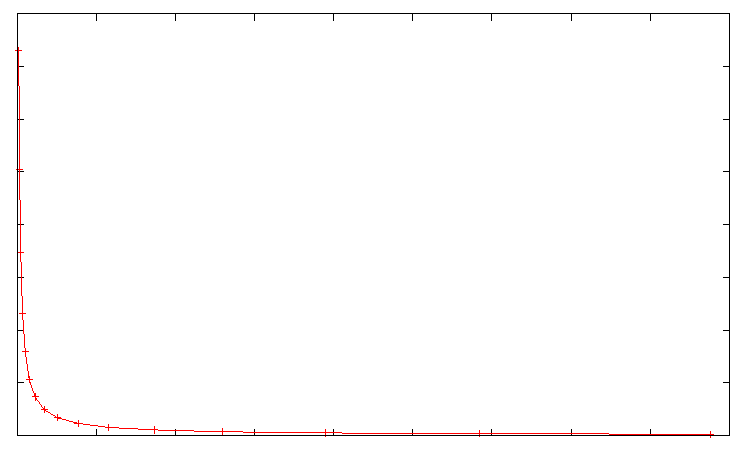
\includegraphics[width=0.23\columnwidth]{flog2-n.pdf} &
    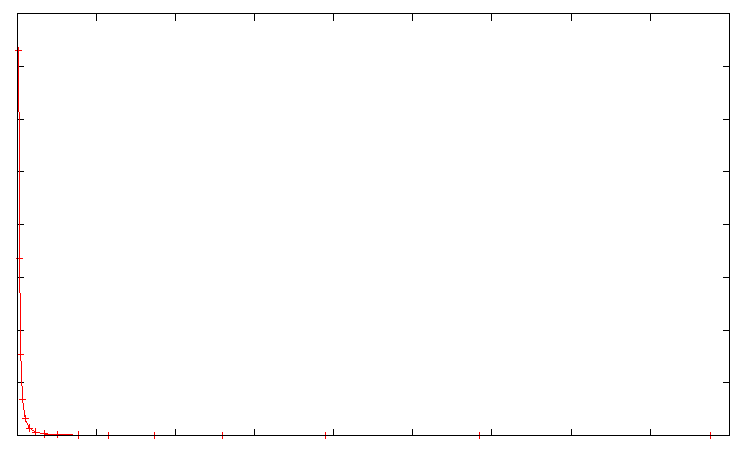
\includegraphics[width=0.23\columnwidth]{flog2-n2.pdf} \\
    \midrule
    \multicolumn{4}{l}{Program \textbf{E}} \\
    \quad
    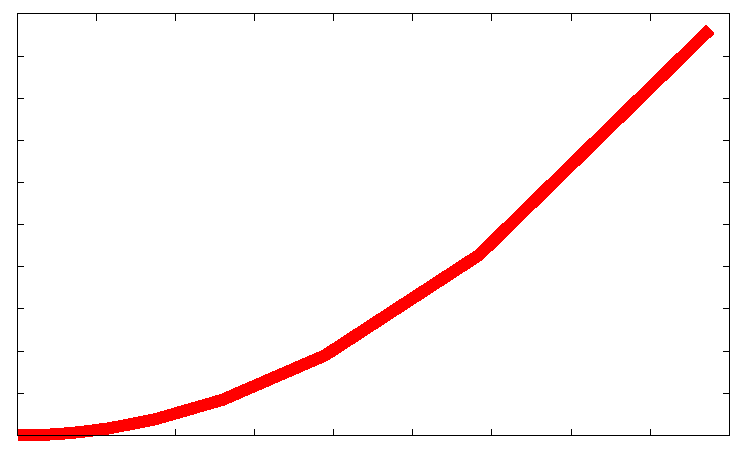
\includegraphics[width=0.23\columnwidth]{fn2.pdf} &
    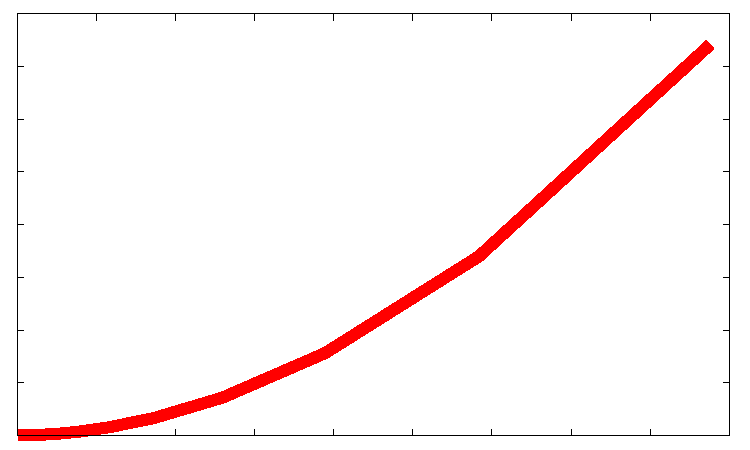
\includegraphics[width=0.23\columnwidth]{fn2-log.pdf} &
    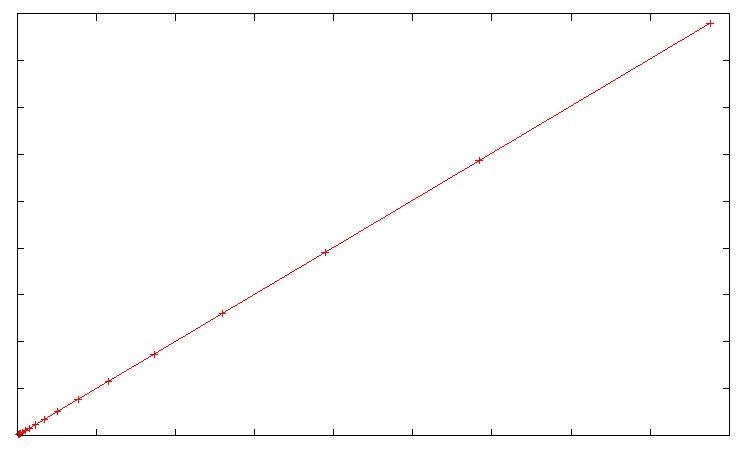
\includegraphics[width=0.23\columnwidth]{fn2-n.pdf} &
    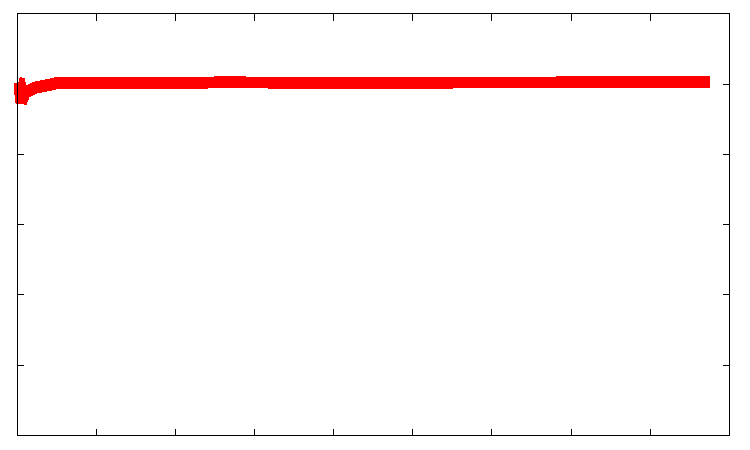
\includegraphics[width=0.23\columnwidth]{fn2-n2.pdf} \\
    \midrule
    \multicolumn{4}{l}{Program \textbf{F}} \\
    \quad
    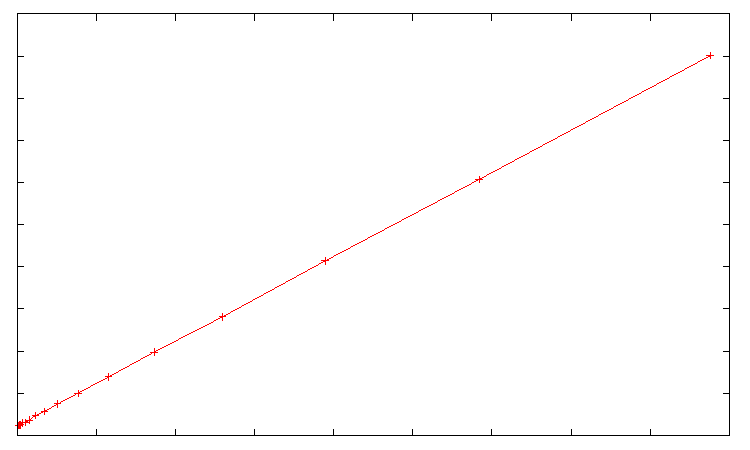
\includegraphics[width=0.23\columnwidth]{flin2.pdf} &
    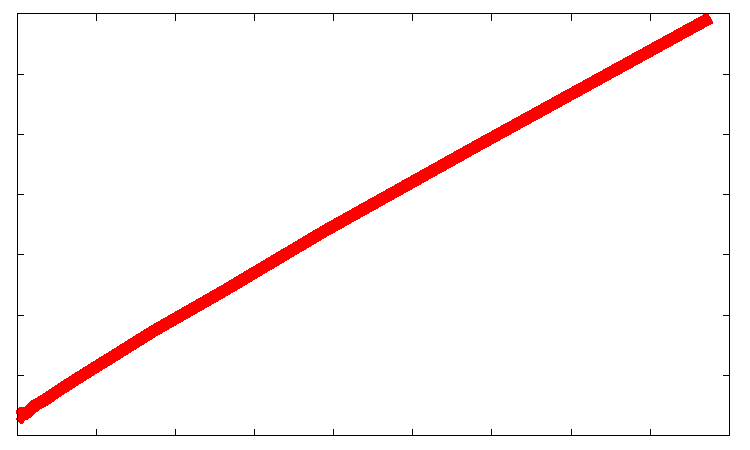
\includegraphics[width=0.23\columnwidth]{flin2-log.pdf} &
    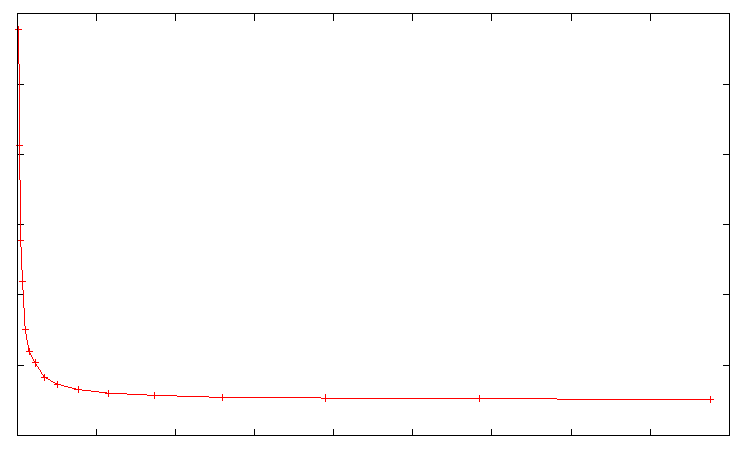
\includegraphics[width=0.23\columnwidth]{flin2-n.pdf} &
    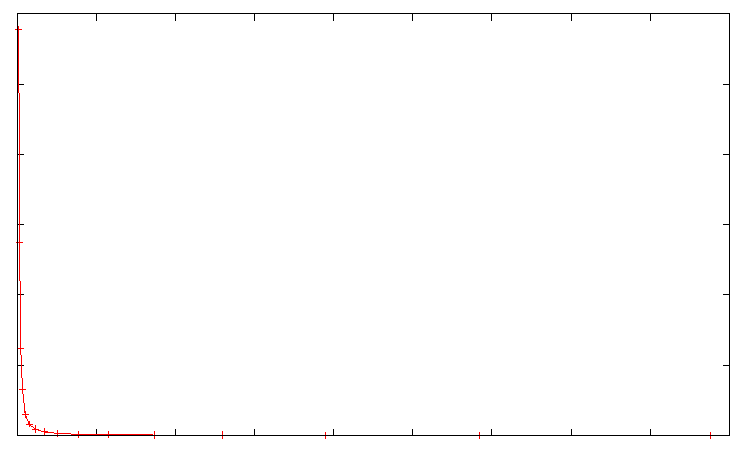
\includegraphics[width=0.23\columnwidth]{flin2-n2.pdf} \\
    \bottomrule
  \end{tabular}
\end{center}



\clearpage
\question{5 points}

\begin{enumerate}
\item
  Draw a diagram of the binary search tree that gets created by the following sequence of insertions:
  \textbf{5, 4, 2, 6, 3, 1, 7}
\item
  In what sequence are these number visited by \textbf{pre-order} traversal?
\item
  What is the sequence when we use \textbf{post-order} traversal?
\item
  What is the sequence with \textbf{in-order} traversal?
\item
  And finally, what sequence results when we use \textbf{level-order} traversal?
\end{enumerate}



\clearpage
\question{4 points}

Knowing the ``Big-Oh'' complexity class of a program's running time $T$ in function of problem size $N$, written $T(N)\in O(F(N))$, allows us to estimate two kinds of things.

\begin{itemize}
\item
  Runtime prediction: if we know that the program took $T_1$ time to run on a problem of size $N_1$, then we can estimate the time $T_2$ required to solve a problem of size $N_2$.
\item
  Problem size prediction: if, on the other hand, we are given a runtime budget of $T_2$, we can estimate the corresponding problem size $N_2$ (again assuming that we know the time $T_1$ for the known problem size $N_1$).
\end{itemize}

Write down the formulas which allow you to solve the \textbf{runtime prediction} problem for the following complexity classes:

\begin{itemize}
\item
  $\log N$
\item
  $N^2\log N$
\item
  $N^3$
\item
  $2^N$
\end{itemize}

Then write down the formulas to solve the \textbf{problem size prediction} problem for the following complexity classes:

\begin{itemize}
\item
  $\log N$
\item
  $N$
\item
  $N^2$
\item
  $2^N$
\end{itemize}



\end{document}
